% !TEX root = WWW.tex
\begin{figure*}[!ht]
\centering
\subfloat[\small \textsc{enron}]{
    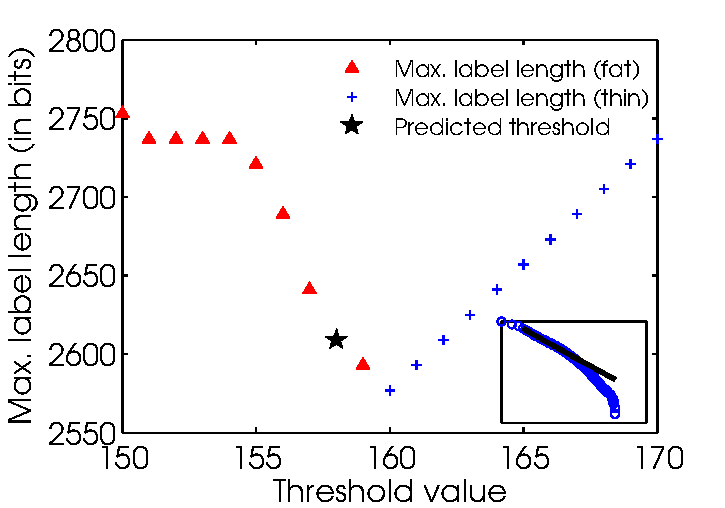
\includegraphics[width=0.32\textwidth]{Figures/enron-modified.pdf}
}
\subfloat[\small \textsc{internet}]{
    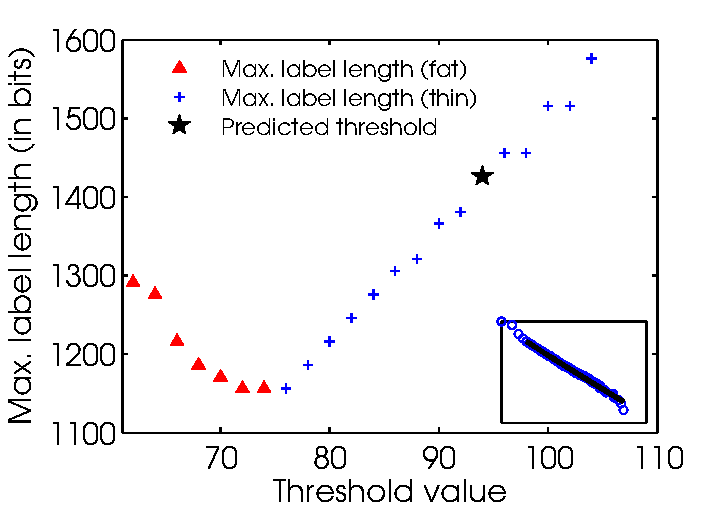
\includegraphics[width=0.32\textwidth]{Figures/internet-modified.pdf}
}%
\subfloat[\small \textsc{www}]{
    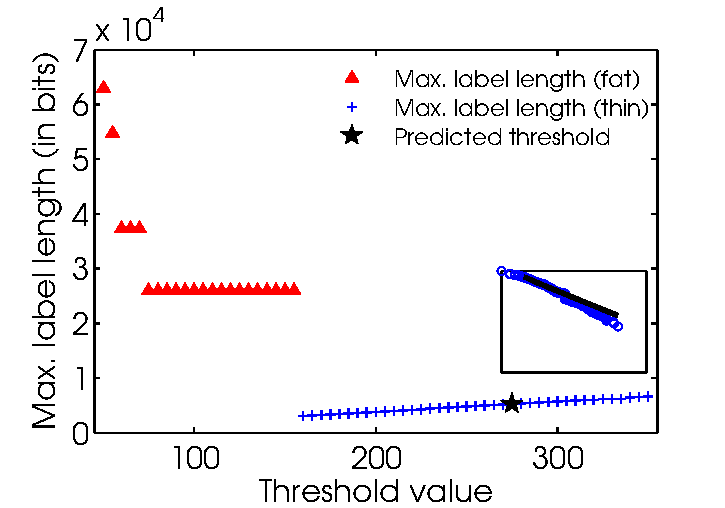
\includegraphics[width=0.32\textwidth]{Figures/www-modified.pdf}
}%
\caption{Predicted and empirical thresholds for the \textsc{enron}, \textsc{internet} and \textsc{www} datasets. The inset show the MLE fitted power law, using the method of Clauset et al.\ \cite{clauset2009power}, where data points are blue circles and the power law is shown as a black solid. The exponents of the power laws are shown in Table \ref{t:datasets}.}%
\label{f:bla}%
\end{figure*}